Quando si parla di simmetrie discrete si mette in enfasi il rapporto tra simmetrie e la classificazione degli stati. Ad esempio la Partità $P$, la coniugazione di carica $C$ e l'inversione temporale. Ognuno presenta possibili autovalori, numeri quantici dei sistemi fermione-antifermione e strumenti che utilizzeremo per classificare in futuro nuove particelle. Vedremo anche la violazione delle simmetrie $P$ e $C$ nelle interazioni deboli. 
\subsection{Simmetrie in meccanica quantistica}
L'evoluzione temporale del valore di aspettazione di una variabile $Q$ è data dal suo commutatore con l'Hamiltoniana
\begin{equation*}
    \frac{d}{dt}\langle Q\rangle=\frac{1}{i\hbar}\langle [Q,H]\rangle
\end{equation*}
In particolare Q è una quantità conservata se e soltanto se: $[Q,H]=0$. In questo caso l'applicazione di una trasformazione $U$, lascia invariata l'Hamiltoniana se:
\begin{equation*}
    UHU^{-1}=H \quad \Rightarrow \quad UH=HU \quad \Rightarrow \quad [U,H]=0
\end{equation*}
In generale se una trasformazione infinitesima si può scrivere:
\begin{equation*}
    U=\text{exp}(-i\hbar\varepsilon G)
\end{equation*}
Dove $G$ è un operatore ed è il generatore di quella trasformazione. Questo $G$ è una quantità conservata perchè se $U$ commuta con l'Hamiltoniana anche $G$ stesso lo fa.
\subsection{Simmetrie e autovalori}
Dalla relazione di commutazione segue che $\psi$ è autostato di $H$, anche $G_\psi$ lo è:
\begin{equation*}
    H(G\psi)=(HG)\psi=(GH)\psi=E_\psi G\psi
\end{equation*}
Se $\psi$ è unico, allora necessariamente deve anche essere autostato di $G$: $G\psi=\eta_G\psi$. Se un certo livello energetico ha $n$ autostati degeneri. Il trasformato di un autostato deve potersi esprimere come sovrapposizione lineare degli altri:
\begin{equation*}
    G\psi_i=\sum_{M=1,\ldots,n}G_{m,i}\psi_m\qquad G_{m,i}=\langle\psi_m|G|\psi_i\rangle
\end{equation*}
diagonalizzando la matrice $G_{m,i}$, si può creare una base di autostati sia di $G$ che di $H$. \textbf{Gli autovalori di G possono venire usati per classificare gli autostati di H}. Ad esempio una particella in un potenziale a simmetria sferica: sono conservati $L^2$ e $L_x,L_y,L_z$ separatamente (generatori delle rotazioni). Gli autovalori della Hamiltoniana dipendono da $L^2$ con degenerazione $n=2l+1$. Solitamente si scelgono come base autofunzioni con le armoniche sferiche. Uso la simmetria per classificare le soluzione dell'equazione di Schr\"odinger.
\subsection{Simmetrie discrete}
Oltre alle trasformazione continue, in meccanica quantistica hanno particolare importanza le trasformazioi discrete: 
\begin{itemize}
    \item Parità $P$: $\mathbf{r}\xrightarrow[]{P}-\mathbf{r}$;
    \item Inversione temporale $T$: $t\xrightarrow[]{T}-t$;
    \item Coniugazione di carica $C$: scambio di particelle con anticoarticelle, non ha un analogo classico.
\end{itemize}
Tutti questi operatori hanno la proprietà di essere idem-potenti: $P^2=T^2=C^2=1$. I possibili autovalori sono quindi solo $1$ e $-1$.
\subsection{Parità}
Grandezze vettoriali possono comportarsi diversamente per trasformazioni di parità:
\begin{itemize}
    \item Vettori polari: cambiano segno per parità. Ad esempio il vettore di coordinate cambia segno per definizione in trasformazione di parità. Allo stesso modo la velocità ed il vettore momento.
    \item Vettori assiali: non cambiano segno per parità. Ad esempio: il momento angolare (questo perchè quando applico l'operatore parità cambia segno la posizione e la quantità di moto), lo spin e anltre grandezze di questo tipo.
\end{itemize}
Analogamente esistono anche:
\begin{itemize}
    \item Grandezze scalari: non cambiano segno per parità.
    \item Grandezze pseudoscalari: cambiano segno per parità. Ad esempio il prodotto scalare tra una quantità di moto e lo spin. In quanto il primo è un vettore polare il secondo è assiale e quindi c'è un effettivo cambio di segno.
\end{itemize}
Nel caso di una partiella in un campo centrale:
\begin{equation*}
    \psi_{n,l,m}=\frac{u_{n,l}(r)}{r}Y_{l,m}(\theta, \phi)
\end{equation*}
Le armoniche sferiche sono tali che la parità applicata alla mia funzione d'onda agisce solo sull'armonica sferica cambiandomi solo l'angolo del vettore:
\begin{equation*}
    P\left[\frac{u_{n,l}(r)}{r}Y_{l,m}(\theta,\phi)\right]=\frac{u_{n,l}(r)}{r}Y_{l,m}(\pi-\theta, \phi+\pi)=(-1)^l\frac{u_{n,l}(r)}{r}Y_{l,m}(\theta,\phi)
\end{equation*}
In aggiunta possiamo assumere che una particella abbia una parità intrinseca, così come ha un momento angolare intrinseco. Per cui la parità di una particella sarà data dalla parità del momento angolare per la parità intrinseca della partiella:
\begin{equation*}
    P\psi_{n,l,m}=\eta_\psi(-1)^l\psi_{n,l,m}
\end{equation*}
Nel caso di due particelle ed una interazione a simmetria sferica, il problema è esattamente analogo a quello di una particella singola, a patto di prendere la massa ridotta:
\begin{equation*}
    P\psi_{n,l,m}=\eta_1\eta_2(-1)^l\psi_{n,l,m}
\end{equation*}
Una volta definita la parità di una certa particella si possono ricavare le altre parità relativa a partire da questa. 
\subsubsection{Parità del campo elettromagnetico}
Il campo elettrico $\mathbf{E}$ è un vettore polare: $P(\mathbf{E}=-\mathbf{E})$. Il campo magnetico $\mathbf{B}$ invece è un vettore assiale: $P(\mathbf{B})=\mathbf{B}$. Le equazioni di Maxwell sono invarianti per trasformazioni di parità:
\begin{equation*}
    \nabla \cdot \mathbf{E}=\frac{\rho}{\varepsilon_0} \qquad  \nabla \cdot \mathbf{B}=0
\end{equation*}
\begin{equation*}
    \nabla \times \mathbf{E}+\frac{\partial \mathbf{B}}{\partial t}=0 \qquad \nabla \times \mathbf{B}-\mu_0 \varepsilon_0 \frac{\partial \mathbf{E}}{\partial t}=\mu_0 \mathbf{J}
\end{equation*}
\textbf{Le interazioni elettromagnetiche conservano la parità}. L'interazione del campo elettromgnetico è di natura polare. Una conseguenza diretta è che il \textbf{fotone ha parità negativa} perchè sostanzialmente tutte le caratteristiche del campo magnetico tutte queste interazioni sono di natura polare.
\subsubsection{Violazione della parità}
Abbiamo appena visto che le interazioni elettromagnetiche conservano la parità. Questo è sperimentalmente osservato che questo vale anche per le interazioni forti. \textbf{Non è così per le interazioni deboli}. L'osservazione sperimentale si basa sulla misura del valore di aspettazione di un'osservabile pseudoscalare $S$:
\begin{equation*}
    S\xrightarrow[]{P}-S
\end{equation*}
Se $P$ è una simmetria, il valore di aspttazione prima e dopo l'applicazione della trasformazione deve coincidere:
\begin{equation*}
    \langle S \rangle \xrightarrow[]{P}\langle -S \rangle=-\langle S \rangle
\end{equation*}
Quindi se $P$ è una simmetria:
\begin{equation*}
    \langle S \rangle=-\langle S \rangle=0
\end{equation*}
Quindi il metodo con cui si è andato a vedere che le interazioni deboli violano la parità non è tanto guardare il fatto che uno stato cambi di parità tanto piuttosto che ho un'osservabile di aspettazione il cui valore è diverso da $0$.
\subsubsection{Esperimento di Wu et al.}
L'esperimento, fatto nel 1956, che ha osservato per la prima volta la relazione di parità. Lo spin dei nuceli del $\ch{^{60}Co}$ è allineato al campo magnetico $\mathbf{B}$. L'idea di base è che voglio andare a vedere un'osservabile pseudoscalare tra la quantità di moto e il campo magnetico. Perchè il campo magnetico è un vettore assiale, la quantità di moto è polare e il loro prodotto scalare è una variabile pseudoscalare. Per fare ciò è necessario raggiungere basse temperature ($\sim10^{-3}K$). L'agitazione termica mi mescola le varie orientazioni perchè la probabilità di essere allineati o meno dipende dall'energia termica. Quindi ho bisogno di un $kT$ sia dell'ordine di grandezza del magnetone nucleare ($\mu_N=3\times10^{-8}\,eV/T$). La violazione di parità tramite osservazione di una correlazione con $\mathbf{B}$ degli elettroni emessi:
%IMMAGINE hg
\begin{figure}[htp!]
  \centering
  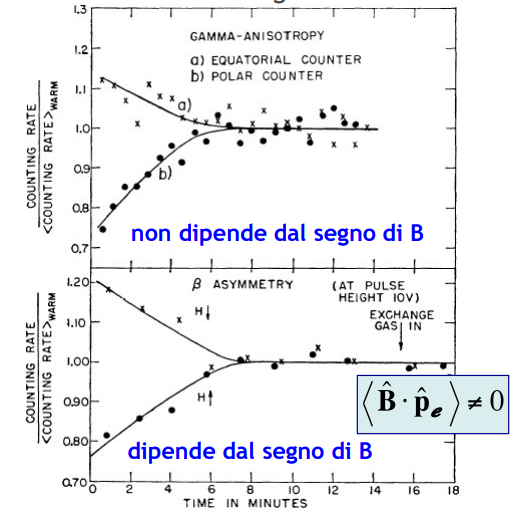
\includegraphics[scale=0.8]{Lezione12/hg.png} 
\end{figure}
Riassunto dell'esperimento per dimostrare che la parità non è una simmetria delle interazioni deboli: abbiamo preso un processo debole e visto che una quantità pseudoscalare aveva valore medio nullo. Siccome, se abbiamo una simmetria di una certa interazione se la applico non dovrebbe cambiare nulla. Una variabile pseudoscalare se applico la parità dovrebbe cambiare di segno e quindi l'unico valore ammesso per rispettare la parità è che il valore sia zero. Ma se come quantità pseudoscalare prendo il momento di un elettrone scalare il campo magnetico scopriamo che questo ha un valore medio diverso da zero in particolare minore di uno. Non ci dice di quanto è violata ma ci dice che non può essere una simmetria dell'interazione debole.
\subsection{Elicità}
Una particolare variabile \textbf{pseudoscalare} è l'elicità:
\begin{equation*}
    h=\frac{\mathbf{p}\cdot\mathbf{S}}{|\mathbf{p}||\mathbf{S}|}=\hat{\mathbf{p}}\cdot\hat{\mathbf{S}}
\end{equation*}
Per particelle di spin $1/2$: $h=1$, se ho lo spin orientato nella direzione del moto o $h=-1$ per lo spin orientato in direzione opposta alla direzione del moto. Il valor medio di $h$ corrisponde ad una polarizzazione netta lungo la direzione del moto:
\begin{equation*}
    \langle \hat{\mathbf{p}}\cdot\hat{\mathbf{S}}\rangle =\frac{N_{h=+1}-N_{h=-1}}{N_{h=+1}+N_{h=-1}}
\end{equation*}
Misure di polarizzazione delle particelle partecipanti ad interazioni deboli mostrano:
\begin{equation*}
    \langle \hat{\mathbf{p}}_{e^-}\cdot\hat{\mathbf{S}}_{e^-}\rangle =-\beta \qquad \langle\hat{\mathbf{p}}_{e^+}\cdot\hat{\mathbf{S}}_{e^+}\rangle =+\beta
\end{equation*}
\begin{equation*}
    \langle \hat{\mathbf{p}}_{\nu}\cdot\hat{\mathbf{S}}_{\nu}\rangle =-1 \qquad \langle\hat{\mathbf{p}}_{\Bar{\nu}}\cdot\hat{\mathbf{S}}_{\Bar{\nu}}\rangle =1
\end{equation*}
Questa misure dimostrano un'altra volta un valore non nullo per una quantità pseudoscalare (prodotto scalare tra vettore polare e vettore assiale) e quindi un'ulteriore conferma alla violazione di $P$. Il fatto che i neutrini abbiamo un'elecità definita presenta una \textbf{violazione massimale} della parità: nel senso che questa variabile pseudoscalare assume il suo valore massimo possibile. Questo si traduce anche in  caratterizzazione dello spettro delle particelle. Ad esempio se prendo un neutrino e applico l'operatore parità lo trasformo in un neutrino con elicità positiva:
\begin{equation*}
    P(\nu_{h=-1})=\cancel{\nu_{h=+1}} \qquad P(\Bar{\nu}_{h=+1})=\cancel{\Bar{\nu}_{h=-1}}
\end{equation*}
che non esistono! Infatti non esistono neutrini con elicità positiva e non esistono antineutrini con elicità negativa. Applico l'operatore parità ad un oggetto e ottengo un insieme vuoto.
\subsection{Coniugazione di carica}
L'operatore di coniugazione di carica $C$ scambia particelle con le rispettive antiparticelle: 
\begin{equation*}
    C(e^-)=e^+ \qquad C(e^+)=e^-
\end{equation*}
\textbf{Tutti i numeri quantici vengono invertiti} non solo la carica. Quindi anche il numero barionico, momento magnetico e spin. Come per la parità si ha che gli autovalori possibili sono $\eta_C=\pm1$. Solo gli stati \textbf{completamente} (sia dal punto di vista elettrico ma anche di tutti le altre cariche) \textbf{neutri} possono essere autostati di $C$. Infatti il neutrone non lo è. $C$ del fotone: $C$ inverte le cariche del sistema: tutti i campi $\mathbf{E}$ e $\mathbf{B}$ cambiano segno. 
\begin{equation*}
    C(\gamma)=-\gamma
\end{equation*}
\subsection{Positronio}
Questo è uno stato legato elettrone-positrone. L'equazione di Schr\"odinger è identica a quella dell'atomo di indrogeno l'unica differenza è la massa ridotta del sistema:
\begin{equation*}
    \mu=\frac{m_em_e}{m_e+m_e}=\frac{m_e}{2}
\end{equation*}
Ci sono quattro possibili configurazioni di spin, si combinano in:
\begin{itemize}
    \item un tripletto con: $S=1$, $S_z=+1,0,-1$;
    \item un singoletto con $S=0$
\end{itemize}
Quale è la parità di questo sistema? In questo caso consiste nello scambiare le posizioni di elettrone e positrone, mentre la coniugazione di carica consiste nello scambiare l'elettrone e il positrone. Sembrano simili ma non sono uguali. Parità: scambio della posizione relativa delle particelle, parità intrinseca.
\begin{equation*}
    \eta_P=\eta_{e^-}\eta_{e^+}(-1)^l
\end{equation*}
La coniugazione di carica: lo scambio di particelle corrisponde alla trasformazione di parità. Ma in più vediamo che può cambiare la funzione di spin: $-1$ per $S=0$, $+1$ per $S=1$ questo perchè se guardo la funzione d'onda e scambio le frecce per $S=1$ scambiare positrone con elettrone mi porta ad avere la stessa identica funzioni d'onda mentre per $S=0$ scambiare elettrone con positrone mi da la stessa funzione d'onda ma con un meno davanti:
%IMMAGINE hg
\begin{figure}[htp!]
  \centering
  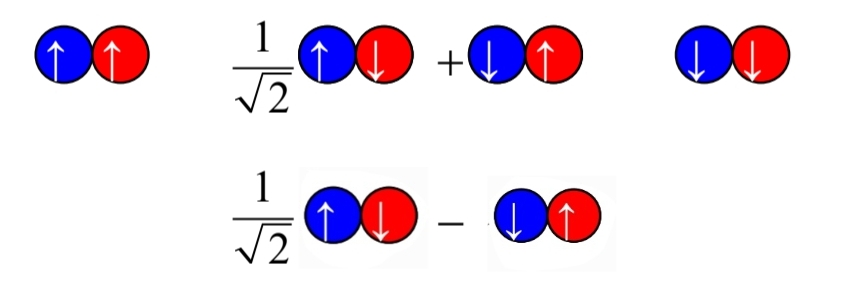
\includegraphics[scale=0.3]{Lezione12/dsad.jpg} 
\end{figure}
\begin{equation*}
    \eta_C=\eta_P(-1)^{S+1}
\end{equation*} 
Quindi l'autovalore di coniugazione di carica è uguale all'autovalore di della parità con un altro fattore che tiene conto del discorso precedente. Lo stato fondamentale ha $l=0$ (per avere energia più bassa in quanto non c'è potenziale centrifugo). Può trovarsi in uno stato di singoletto: \textbf{para-positronio} $\ch{^1S_0}$ (con spin totale $S=0$) e lo stato di tripletto: \textbf{orto-positronio} $\ch{^3S_1}$ (con spin totale $S=1$). I due stati hanno la stessa parità in quanto dipende solo da $l$ e non da $S$: $\eta_P=\eta_{e^-}\eta_{e^+}$ anche se i livelli differiscono di $8\times10^{-4}\,eV$ non si può transire elettromagneticamente: emissione di un $\gamma$ cambia parità $\eta_\gamma=-1$ per cui se passiamo da uno stato all'altro siamo obbligati a cambiare parità perchè il fotone esce con parità negativa e quindi questa transizione è proibita perchè violerebbe la parità. Due stati quasi-stabili. Elettrone e positrone girano attorno per un po' fino a quando si incontrano e si annichilano. 

Però hanno una coniugazione di carica opposta: $\eta_C=\eta_P(-1)^{S+1}$. Il para-positronio decade in $125\,ns$ in uno stato con $2\gamma$: $\eta_C=+1$ (questo perchè ogni fotone ha coniugazione di carica negativa e quindi se ne escono due abbiamo una coniugazione di carica positiva che deve conservarsi). L'orto-positronio decade in $140\,\mu s$ in uno stato con $3\gamma$: $\eta_C=-1$. Questo implica che $\eta_P=\eta_{e^+}\eta_{e^-}=-1$ e che quindi \textbf{parità di fermione ed antifermione sono opposte}. I fermioni sono una specie di particelle davvero carognosa: non vogliono stare insieme (Principio di esclusione di Pauli), hanno una funzione d'onda antisimmetrica, hanno parità opposta, quando faccio rotazione di $360^\circ$ cambiano segno.

Il risultato, al pari di $g=2$, predetto dalla meccanica quantistica relativistica. C'è un altro modo per verificare la parità di questi stati e cioè verificare direttamente dallo studio della correlazione tra le polarizzazioni di $\varepsilon_1$ e $\varepsilon_2$ dei fotoni uscenti dal decadimento del parapositronio, discriminando i casi.
Quale dei due ha parità negativa o positiva è convenzionale.
\subsection{Violazione della coniugazione di carica}
Nelle interazioni deboli viene anche violata $C$, sempre nel caso del neutrino:
\begin{equation*}
    C(\nu_{h=-1})=\cancel{\Bar{\nu}_{h=-1}}
\end{equation*}
Che non esiste. Tuttavia funziona la trasformazione composta:
\begin{equation*}
    CP(\nu_{h=-1})=C(\nu_{h=+1})=\Bar{\nu}_{h=+1}
\end{equation*}
Quindi $CP$ risulta una simmetria più fondamentale di $C$ e $P$ separatamente. Vedremo che anch'essa sarà violata dalle interazioni deboli, ma ad un livello decisamente minore.
\subsection{Inversione temporale}
Classicamente l'operatore di inversione temporate $T$: $t\to-t$. La versione quantistica è tale che:
\begin{equation*}
    T\psi(\mathbf{r},t)=\psi^*(\mathbf{r},-t)
\end{equation*}
Partendo dall'equazione di Schr\"odinger:
\begin{equation*}
    i\hbar\frac{\partial\psi(\mathbf{r},t)}{\partial t}=H\psi(\mathbf{r},t)
\end{equation*}
Facendo il coniugato:
\begin{equation*}
    -i\hbar\frac{\partial\psi^*(\mathbf{r},t)}{\partial t}=H\psi^*(\mathbf{r},t)
\end{equation*}
E poi l'inversione temporale $t\to-t$:
\begin{equation*}
    i\hbar\frac{\partial\psi^*(\mathbf{r},-t)}{\partial t}=H\psi^*(\mathbf{r},-t)
\end{equation*}
$\psi^*(\mathbf{r},t)$ è soluzione dell'equazione di Schr\"odinger con la stessa energia di $\psi(\mathbf{r},t)$ se $THT^{-1}=H$. Sotto $T$ cambiano di segno $\mathbf{v}$, $\mathbf{p}$. $\mathbf{L}$, $\mathbf{S}$. Esempio particella libera:
\begin{equation*}
    \psi(\mathbf{p})=e^{\frac{i}{\hbar}(\mathbf{p}\cdot\mathbf{r}-Et)} \quad \to \quad \psi^*(\mathbf{p})=e^{-\frac{i}{\hbar}(\mathbf{p}\cdot\mathbf{r}-Et)} \quad \to \quad T\psi(\mathbf{r})=e^{\frac{i}{\hbar}(-\mathbf{p}\cdot\mathbf{r}-Et)}=\psi(-\mathbf{p})
\end{equation*}
Si può fare lo stesso discorso per il momento angolare.
\subsection{Principio del bilancio dettagliato}
Una conseguenza significativa dell'invarianza temporale è l'invarianza dell'elemento di matrice:
\begin{equation*}
    \langle f|U|i\rangle=\int d\mathbf{r}\psi_f^*(\mathbf{r})U(\mathbf{r})\psi_i(\mathbf{r})\xrightarrow[]{T}\int d\mathbf{r}\psi_f(\mathbf{r})U(\mathbf{r})\psi_i^*(\mathbf{r})= \langle i|U|f\rangle
\end{equation*}
Nella probabilità di transizione:
\begin{equation*}
    P(f\to i)=\frac{2\pi}{\hbar}|\langle f|U|i\rangle|^2\rho(E_f)
\end{equation*}
\begin{equation*}
    P(i\to f)=\frac{2\pi}{\hbar}|\langle i|U|f\rangle|^2\rho(E_i)
\end{equation*}
Se vale l'invarianza per inversione temporale: $\langle f|U|i\rangle=\langle i|U|f\rangle$ e quindi la differenza di probabilità è dovuta solamente ai termini di densità di stati. In una situazione di equilibrio: il numero di particelle in un certo stato deve rimanere costante
\begin{equation*}
    \frac{dN_f}{dt}=N_iP(i\to f)-N_fP(f\to i)=0
\end{equation*}
Dove ovviamente il primo termine indica le particelle che passato da uno stato $i$ a uno stato $f$ a cui devo togliere tutti gli stati che passano dallo stato $f$ allo stato $i$. Quando chiediamo questo abbiamo che il rapporto tra il rapporto delle popolazioni è:
\begin{equation*}
    \frac{N_i}{N_f}=\frac{P(f\to i)}{P(i\to f)}=\frac{\rho(E_i)}{\rho(E_f)}
\end{equation*}
\textbf{Principio del bilancio dettagliato} che si userà per misurare lo spin del pione.
\subsection{Invarianza di crossing}
Il principio del bilancio dettagliato viene spesso applicato insieme all'invarianza di crossing: reazioni derivate spostando una particella da stato iniziale a stato finale (o viceversa) e trasformandola in antiparticella. Se una reazione è possibile anche le altre lo sono. Esempio:
\begin{equation*}
    A+B\to C+D
\end{equation*}
Questa transizione, la sezione d'urto di questa transizione viene da un elemento di matrice che sarà in funzione dei vari momenti: $M(\mathbf{p}_A,\mathbf{p}_B,\mathbf{p}_C,\mathbf{p}_D)$. Allora:
\begin{equation*}
    A\to\Bar{B}+C+D \text{ con } M(\mathbf{p}_A,-\mathbf{p}_B,\mathbf{p}_C,\mathbf{p}_D)
\end{equation*}
Posso fare la stessa cosa per tutti gli elementi. Il tasso delle reazioni è poi determinato dal termine di densità degli stati. 
\subsection{Decadimento beta inverso}
(anti)neutrini vengono prodotti dai decadimenti $\beta^\pm$:
\begin{equation*}
    \ch{^A_ZX}\to \ch{^A_{Z-1}X'}+e^++\nu \qquad   \ch{^A_ZX}\to \ch{^A_{Z+1}X'}+e^-+\Bar{\nu}
\end{equation*}
Dove il $Q$-valore della relazione è:
\begin{equation*}
    Q=M(A,Z)-M(A,Z\pm1)-m_e \text{ masse nucleari }
\end{equation*}
I processi di interazione si ottengono applicando prima di tutto l'inversione temporale:
\begin{equation*}
    \ch{^A_{Z-1}X'}+e^++\nu\to\ch{^A_ZX} \qquad  \ch{^A_{Z+1}X'}+e^-+\Bar{\nu}\to\ch{^A_ZX}
\end{equation*}
e quindi il nucleo con $(A,Z\pm1)$ cattura un positrone/elettrone ed un neutrino/antineutrino e si trasforma nel nucleo con $(A,Z)$. Successivamente posso utilizzare l'invarianza di crossing:
\begin{equation*}
    \ch{^A_{Z-1}X'}+\nu\to\ch{^A_ZX}+e^- \qquad  \ch{^A_{Z+1}X'}+\Bar{\nu}\to\ch{^A_ZX}+e^+
\end{equation*}
L'elemento di matrice del decadimento $\beta$:
\begin{equation*}
      \left\langle f\left|H_W\right| i\right\rangle =\frac{G_F(\hbar c)^3}{V} \int_V d \mathbf{r}\left(\psi_{A, Z+1}(\mathbf{r}) \psi_e(\mathbf{r}) \psi_\nu(\mathbf{r})\right)^* O_X \psi_{A, Z}(\mathbf{r})=\frac{G_F(\hbar c)^3}{V}M_{fi}
\end{equation*}
si applica anche al decadimento $\beta$ inverso, dall'espressione della larghezza di decadimento:
\begin{equation*}
    \Gamma=\frac{\hbar}{\tau}=\frac{G_F^2|M_{fi}|^2(m_ec^2)^5}{2\pi^3}f(Z,Q)
\end{equation*}
con
\begin{equation*}
    f(Z, Q)=\int_0^{Q / m_e c^2} d\left(\frac{T_e}{m_e c^2}\right) \frac{p_e}{m_e c}\left(1+\frac{T_e}{m_e c^2}\right)\left(\frac{Q-T_e}{m_e c^2}\right)^2 F\left(Z, T_e\right)
\end{equation*}
e quindi:
\begin{equation*}
    |\langle f|H_W|\rangle|^2=\Gamma\frac{(\hbar c)^6}{V^2}\frac{2\pi^3}{(m_e c^2)^5f(Z,Q)}
\end{equation*}
Calcoliamo la sezione d'urto del decadimento $\beta$ inverso. L'espressione per il tasso di transizione:
\begin{equation*}
    \lambda=\frac{2\pi}{\hbar}|\langle f|H_W|\rangle|^2\rho(E_f)
\end{equation*}
Il termine di densità di stati, se trascuriamo la piccola quantità di energia portata via dal nucleo:
\begin{equation*}
    \rho(E_f)=\frac{dN}{dE_f}=\frac{V\times4\pi p_e^2}{(2\pi\hbar)^3}\frac{dp_e}{dE_f}\xrightarrow[]{(pc)d(pc)=EdE}\frac{V\times4\pi p_e E_e}{(2\pi\hbar)^3c^2}\frac{dE_e}{dE_f}=\frac{V\times4\pi\beta_eE^2_e}{(2\pi\hbar c)^3}
\end{equation*}
Perchè so che $\frac{dE_e}{dE_f}=1$ perchè l'energia dello stato finale è l'energia dell'elettrone visto che si porta via tutta l'energia. Dove $E_e=E_\nu-Q-m_e$. Dalla condizione $E_e\ge m_e$, abbiamo l'energia di soglia del neutrino: $E_\nu>Q+2m_e$. Tenendo conto dell'energia del nucleo la relazione relativistica è corretta da un ulteriore fattore.

Il tasso di transizione:
\begin{equation*}
    \lambda=\frac{2\pi}{\hbar}\frac{(\hbar c)^6}{V^2}\frac{2\pi^3\hbar}{(m_ec^2)^5\tau f(Z,Q)}\frac{V\times 4\pi\beta_eE_e^2}{(2\pi\hbar c)^3}=2\pi^2\frac{(\hbar c)^3}{V}\frac{\beta_e E_e^2}{(m_ec^2)^5\tau f(Z,Q)}
\end{equation*}
La probabilità di transizione da neutrino e nucleo a elettrone e nucleo. Confrontando con la relazione per la sezione d'urto:
\begin{equation*}
    \frac{dn}{dt}=I_0n_Td\sigma
\end{equation*}
Ma nel caso di una particella ho che $dn/dt=\lambda$. Mentre per $I_0$ è un (anti)neutrino che percorre lo spessore $d$ con una velocità $c$: $I_0=c/d$. Mentre un bersaglio nel volume $V$: $n_T=1/V$. In questo caso $\sigma$ vale:
\begin{equation*}
    \sigma=2\pi^2\frac{\beta_eE^2_e}{(m_ec^2)^5f(Z,Q)}\frac{\hbar}{\tau}(\hbar c)^2
\end{equation*}
Dove il primo termine rappresenta il rapporto delle densità degli stati. Quindi è interessante perchè sottolinea come possiamo mettere dei collegamenti tra diversi processi. Conoscendo un processo possiamo stimare le probabilità di un altro processo. 
\subsection{Teorema CPT}
Sta per l'applicazione composta di inversione temporale, parità e coniugazione di carica. Abbiamo visto che $C$ e $P$ sono violate dalle interazioni deboli. Tali simmetrie non sono simmetrie fondamentali della natura. Si può invece dimostrare che una teoria quantistica che è: invariante per trasformazioni di Lorenz, locale, con Hamiltoniana hermitiana. Deve essere invariante rispetto al prodotto delle tre trasformazioni $C$, $P$, $T$. $CPT$ è una simmetrie fondamentale della natura (per le scoperte fino ad esso):
particelle e antiparticelle devono avere la \textbf{stessa massa}, le particelle ed antiparticelle devono avere la \textbf{stessa vita media totale}. Per verificare questa simmetria si effettuano è vedere se le particelle e antiparticelle hanno la stessa massa o la stesssa vita media. Oppure si possono ricercare le violazioni all'invarianza per trasformazioni di Lorentz.